% Chapter 1

\chapter{Introduction} % Main chapter title

\label{Chapter1} % For referencing the chapter elsewhere, use \ref{Chapter1} 

\lhead{Chapter 1. \emph{Introduction}} % This is for the header on each page - perhaps a shortened title

%----------------------------------------------------------------------------------------

\noindent Cloud-based applications are typically large-scale systems that rely on complex software stacks. Managing such applications is not a trivial task, especially if the application spans across multiple cloud providers and different locations \cite{elmroth2011self}. Some of the important challenges during their lifecycle are (i) how to provision and deploy an application and (ii) how to manage its state and evolution. 

There are two main approaches to the resource provisioning and deployment of cloud applications: imperative and declarative. In this work we identify benefits and limitations of each approach with help of the motivating example, and show how a combination of both approaches can benefit application operators. In addition, to make the deployment process as simple as possible, we introduce a domain-specific language for the specification and manipulation of the deployment plans (a set of instructions on how to deploy an application). Using this language we can illustrate the deployment process in real-time, which helps application operators to analyze and optimize the process itself.  

Regarding the application state and evolution, a  common approache is to redeploy the whole application whenever it needs to be updated, another one is to write new updating scripts and execute them each time the running system should be updated. Such solutions are either cumbersome (because application operators have to maintain the list of scripts) or not efficient (because cloud resources must be deprovisioned for the old system and provisioned again for the new one). In this work we show how the usage of the models@runtime pattern in combination with our domain-specific language allows to update applications efficiently and without much effort.

Finally, we conduct a set of deployment experiments to validate and evaluate the proposed solutions.

The results of this thesis are included in the paper to be submitted in the models@runtime workshop at the ACM/IEEE MODELS 2015 conference\footnote{ ACM/IEEE MODELS 2015 conference, http://www.modelsconference.org/}.


%----------------------------------------------------------------------------------------

\section{Research Motivation}

In this section we outline several reasons how the research presented in this paper  addresses important concerns of the cloud application operators.

\subsection{Background}

\noindent As we mentioned earlier, important challenges during the life-cycle of cloud applications include (i) how to provision and deploy an application and (ii) how to manage its state and evolution. 

\noindent Provisioning\footnote{ OGSA Glossary of Terms v.1.6, $  $https://redmine.ogf.org/dmsf\_files/10963?download=} of the application means allocation of the required resources on the chosen cloud. Resources may be virtual machines, storage, load balancers, domain name system (DNS) records and more. Every cloud provider exposes a self-service portal and an Application-Programming Interface (API) that can be exploited to provision cloud resources, but most of those interfaces have different syntax and behavior thus introducing a so-called vendor lock-in. As a result, cloud application providers planning to run different components of their application on different clouds (e.g., a database on Amazon and a web server on Google) have to manage different APIs. This issue has been partially solved by libraries such as jclouds\footnote{ Apache jclouds, $  $http://jclouds.apache.org/} or deltacloud\footnote{ Deltacloud, https://deltacloud.apache.org/ }, which provide a uniform interface to access all major cloud providers. For instance, in jclouds, operators can define minimum RAM and CPU requirements for their virtual machines and it will try to allocate them on the chosen cloud according to cloud provider's capabilities. Nevertheless, when cloud application providers are not limiting themselves to the infrastructure level and want to provision particular application components on Platform-as-a-Service (PaaS),  they have to rely on diverse cloud provider-specific APIs. To handle this heterogeneity a standardization effort has been made which led to the specification of the Cloud Application Management for Platforms (CAMP) standard \cite{CAMP-v1.1}. Still, the challenge remains to provision Infrastructure-as-a-Service (IaaS) and PaaS level application components at the same time.

\noindent 

\noindent Deployment refers to all activities required to make the cloud application ready for use \cite{specification2006deployment}. Deployment activities encompass tasks such as downloading and installing all required software components, configuring them and establishing connections with other relevant components (e.g., connect caching server to the web server). Challenging aspects of the deployment phase are how to ensure the proper order of installation between different components and how to share relevant data between them (e.g., how to configure database URL in the web server if the database is located on the different virtual machine and internet protocol (IP) address of that machine is not known in advance).

\noindent 

\noindent The provisioning and deployment tasks may be done manually or automatically. Manual execution of these tasks is not suitable for large-scale cloud applications because it is error-prone, not time-efficient and hardly feasible if many virtual machines and software packages have to be installed and configured. Therefore, application developers and operators are looking for automation. Automation of these tasks typically has two flavors: declarative and imperative \cite{INPROC-2013-45}. The imperative approach requires the explicit definition of how to reach the desired state of the application in the application deployment plan, usually by means of some general workflow language. The deployment plan is a workflow - a set of atomic tasks that are executed in a specific order (some of them may run in parallel). The imperative approach gives developers full control over the deployment process but reduces the reusability of the solution because writing in the first place and then changing such plans is not a trivial task. In contrast, the declarative approach requires only specification of the desired final state of the application. This state is usually described in the application topology model or blueprint using a domain-specific language (DSL), and then exact steps on how to reach that state will be derived from this model by the deployment engine. Such an approach allows developers to reuse their topology model in different scenarios by doing small updates to the model. Nevertheless, the generation of the deployment plan relies on a set of predefined rules, and since  these rules are typically not subject to change, all possible plans can not be generated. In addition, generated plans may not be optimal because they were generated according to the default rules. ~We will illustrate each approach and their limitations in the motivating example. 

\noindent 

\noindent Application management after the deployment (runtime phase) includes monitoring, error handling, software updates, dynamic reconfiguration and scaling operations. Among the challenging tasks is the dynamic reconfiguration of the system, which may include evaluation of dependencies between system components and their current state, calculation of the required changes to the application, generation of the adaptation plan, and its execution \cite{arshad2007deployment}. Dynamic reconfiguration includes scaling of the application, which may be achieved by moving the application to a more powerful server (scale-up) or by deploying it to multiple interconnected servers, possibly with a load balancer (scale-out) \cite{michael2007scale}. Manually, it could be done by updating the application topology model for instance via API calls to some application manager or via command-line tools if there are any. In automatic way, scalability may be achieved with help of policies that define when the application or some part of it shall be scaled in or out (or up or down), this exploits one of the main features of the clouds called elasticity: ``Elasticity is the degree to which a system is able to adapt to workload changes by provisioning and deprovisioning resources in an autonomic manner, such that at each point in time the available resources match the current demand as closely as possible'' \cite{herbst2013elasticity}. 

\noindent 

\noindent The complexity of specifying application deployment (either via application topology model or deployment plan) and of maintaining and thus dynamically adapting the deployment of cloud application are important challenges faced by cloud application operators. The proposed approach tackles these challenges by enabling the automatic plan generation, based on a declarative specification of the target application topology, and the specification of detailed deployment plans, based on an imperative approach, together with support for the dynamic reconfiguration of the running system in an efficient and controllable manner by exploiting models@runtime technologies.

\noindent 

\noindent In the motivating example we aim to showcase the pros and cons of different deployment approaches and difficulties of management tasks such as dynamic reconfigurations of the deployment of a cloud-based applications. This will provide us with a basis to formulate our research goal.

%----------------------------------------------------------------------------------------

\subsection{Motivating Scenario}

\noindent To have a better understanding of the previously discussed challenges and approaches, the following motivating scenario has been developed: installation of a distributed real-time computation system called Apache Storm\footnote{ Apache Storm, $  $https://storm.apache.org/}. The architecture of the Apache Storm is shown on Figure \ref{fig:Storm}. and in short consists of a master node (nimbus), which assigns tasks to slave nodes (supervisors) whilst all coordination between master and slave nodes is done with help of the Zookeeper\footnote{ Apache Zookeeper, $  $https://zookeeper.apache.org/} cluster (a service which enables reliable distributed coordination). 

\noindent 

\begin{figure}[htbp]
	\centering
		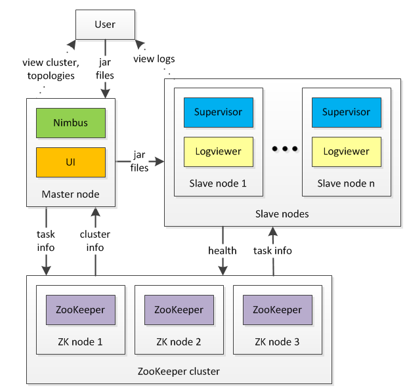
\includegraphics{./Figures/Storm_architecture}
		\rule{38em}{0.5pt}
	\caption[Storm Architecture]{Apache Storm architecture (http://jansipke.nl/storm-in-pictures/)}
	\label{fig:Storm}
\end{figure}

\noindent

\noindent \textbf{\textit{System setup}}. For our scenario, we consider one master node, one zookeeper node, and three slave nodes. Each node is a virtual machine running Ubuntu 14.04 as operating system, the master and slave nodes will be hosted on Amazon EC2\footnote{ AWS Command Line Interface, $  $http://docs.aws.amazon.com/cli/latest/userguide/cli-chap-welcome.html} and zookeeper node on OpenStack\footnote{ OpenStack Command Line Interface, $  $http://docs.openstack.org/cli-reference/content/}. Even for such a simple system, manual provisioning of virtual machines and installation of software components could take from a few hours to one day, assuming the user already knows how to install everything and in which order. In addition, application deployment must be reproducible, which is hardly the case for the manual approach. That is why we need some sort of automation: declarative or imperative. In addition, we will detail the challenges that arise after the application deployment.  

\noindent

\noindent \textbf{\textit{Imperative approach}}. Both Amazon EC2 and OpenStack have a command-line interface (CLI) which can be used for provisioning of virtual machines (APIs could also be used, but for simplicity we went for CLI). So, assuming the command line tools are installed, we could create a bash script or a deployment plan similar to the pseudocode\footnote{ Pseudocode standard, $  $http://users.csc.calpoly.edu/\~{}jdalbey/SWE/pdl\_std.html} depicted in Listing \ref{lst:1}.

\noindent Such plan would automate the whole process of provisioning and deployment of storm cluster on Amazon and OpenStack infrastructures. If we wrap-up part of the code in black font into ``init'' function and the one in blue font into ``add\_slave'' function, we would create management operations which could be used through the life-cycle of our application.

\begin{center}
	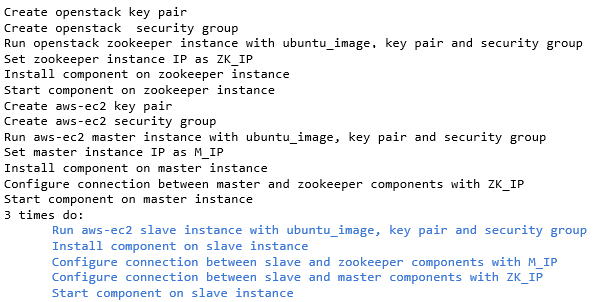
\includegraphics[width=38em]{./Figures/Imperative}
	\begin{lstlisting}[mathescape,caption={Imperative approach to deploy storm cluster},label={lst:1}]
	\end{lstlisting}
\end{center}

\noindent However, what if we would like to run the zookeeper server on Amazon? We would have to rewrite part of the provisioning and deployment plan. Moreover, in the situation when one zookeeper node can not cope with the imposed workload, there is a need to change to a cluster of zookeeper nodes. In that case we would have to change the whole plan because then the master node and every slave node needs to know IP addresses of all zookeeper nodes (also all zookeeper nodes have to know about each other), so the number of connections would grow exponentially. 

\noindent


\noindent Rising these questions shows us that imperative automation approaches handle well provisioning and deployment tasks because developers have fine-grained control of every step in the deployment plan, but they are less reusable and usually tied to one specific scenario.

\noindent 

\noindent \textbf{\textit{Declarative approach}}. As mentioned before, in declarative approaches application operators need to define the structure of the application and then the deployment plan will be derived from that structure and executed in the proper order by the deployment engine. The deployment engine will also take care of the data exchange between different tasks like an exchange of IP addresses of virtual machines. We used CloudML \cite{FerrySongRCS14} as an example of such approach. There we had to describe our desired providers, virtual machines, software components and relations between them. A folded representation of the JSON description of the storm CloudML application topology model from the JSON online editor\footnote{ JSON online editor, https://www.jsoneditoronline.org/} is shown on Figure \ref{fig:JSON}:

\noindent

\begin{figure}[htbp]
	\centering
		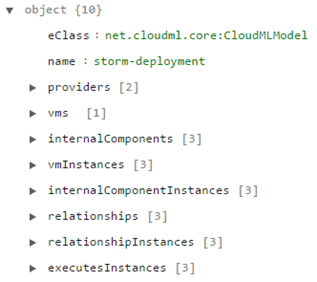
\includegraphics{./Figures/Declarative}
		\rule{38em}{0.5pt}
	\caption[Declarative Approach]{CloudML application model in JSON}
	\label{fig:JSON}
\end{figure}

\noindent

\noindent Providers, vms, internalComponents and relationships sections define reusable types, while other sections - instances of these specific types. The order of provisioning and deployment is based on components' requirements. For instance, zookeeper internal component type requires an Ubuntu based platform as illustrated in Listing \ref{lst:2}:

\begin{center}
	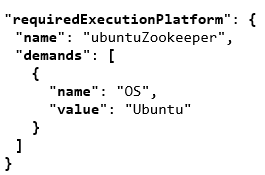
\includegraphics{./Figures/Zookeeper}
	\begin{lstlisting}[caption={Specification of the required platform for Zookeeper component},label={lst:2}]    
	\end{lstlisting}
\end{center}

\noindent It implies that the zookeeper will be executed on a VM running Ubuntu as the operating system and thus that the VM should be provisioned first.

\noindent 

\noindent If we would like to run the zookeeper on Amazon, we would only have to change the provider name of the zookeeper VM. In case of changing from one zookeeper node to a zookeeper cluster, we could use the scale out facilities offered by the DSL. This is similar to management operations that could be created from the imperative script mentioned previously, but in declarative approaches reusability of components is a given feature.

\noindent 

\noindent So, reusability of the application component types and implicit deployment logic (deployment engine deploys the application according to its internal execution rules) are the main advantages of the declarative approaches. Nevertheless, hidden deployment logic also imposes some limitations for the developers, for example, what if the application administrator wanted to change the order of execution for some tasks? This would not be possible due to the deployment engine policies. This pin points the main limitation of declarative approaches: the~lack of flexibility. 

%----------------------------------------------------------------------------------------

\subsection{Discussion}
\label{sec:Discussion}

\noindent As we see from our scenario, imperative approaches are less reusable and involve hard and time-consuming tasks of writing deployment plans \cite{Breitenbuecher2014}, while declarative approaches are less flexible. Another aspect of the deployment phase is the process visibility: in imperative approaches you know exactly how the provisioning and deployment tasks will be performed because you specify the deployment plan yourself, while in declarative the process is hidden from you and in practice you have to imagine it when you design your application topology because components' operations, constraints, capabilities actually represent concrete steps during the provisioning and deployment; also it may be not clear how data is shared between components. 

\noindent 

\noindent One more important aspect that we briefly mentioned before is the dynamic reconfiguration of applications. No matter which deployment automation approach or even combination of them is chosen by the application developers, applications evolve over time and have to be redeployed, often many times. This process should be automated enabling the dynamic reconfiguration of the system, and therefore offering support for what is called ``continuous deployment'': ``Continuous deployment is the practice of continuously deploying good software builds automatically to some environment, but not necessarily to actual users'' \cite{fitzgerald2014continuous}. ~For imperative approaches, this can be achieved by writing additional provisioning and deployment plans and executing them to change the existing application. A drawback of such methodology is that your initial application topology or deployment plan will not be synchronized with changes from additional plans, so if you decided to migrate your application, you would have to replay all plans again in the proper order to reach the same state of the application which means redeployment of the whole application. In declarative approaches, in order to minimize the impact on the running system and thus maximize the application availability, continuous deployment could be achieved by calculating the difference between the previous application topology model and the new one, and then by adapting the running application according to calculated differences as proposed in \cite{FerrySongRCS14}. However, this assumes that the running system is stable. If some virtual machine stopped for any reason, adopting these changes to the previous model would result in the wrong configuration. A simpler scenario would be just to redeploy the whole application, but it is not efficient. A solution to this is to implement the models@run-time architectural pattern. Models@run-time provides an abstract representation of the running application. A change in the running application is immediately propagated to the model of the current system and the same is true for the opposite, any changes to the model are enacted on the running application \cite{FerrySongRCS14}. By using this pattern, application developers can have a consistent view of the system at any time and seamlessly evolve it in the future. To the best of our knowledge, this pattern has been used only in a declarative approach in the context of cloud computing.

\noindent 

\noindent Following the discussion, our proposal for the application provisioning and deployment consists in combining the declarative and imperative approaches: the deployment engine generates the provisioning and deployment plan from the defined application topology model and then the user can analyze it and then has ability to change it before the actual enactment of the plan. Moreover, in case of continuous deployment the same process takes place. For instance, the user changes the topology of an application, an adaptation plan is generated and the user can tune it before the plan will be executed (Figure \ref{fig:solution}). 

\noindent

\begin{figure}[htbp]
	\centering
		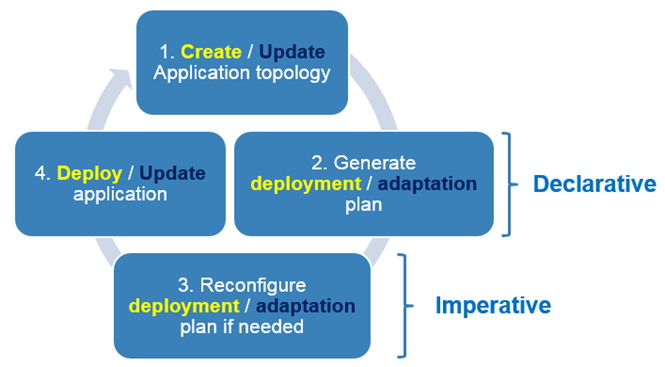
\includegraphics[width=34em]{./Figures/Desired}
		\rule{38em}{0.5pt}
	\caption[Desired Solution]{Desired Solution}
	\label{fig:solution}
\end{figure}

\noindent

\noindent Because imperative approaches often use general workflow languages for the specification of the deployment plan, it would be nice if our plan were expressed using some domain-specific language for modeling workflows.

\noindent In such scenario we preserve reusability of declarative approaches and add flexibility of imperative ones, we have the visibility of the process execution without writing the process ourselves, and we can properly evolve our application and be ready for migration without the issue of replaying a set of workflows or synchronization of our initial application topology with its current state. In addition, this approach results in the reduced time-to-market and development efforts.

%----------------------------------------------------------------------------------------

\section{Research Problem}

\noindent In this work we focus on two challenges: (i) combination of the declarative and imperative approaches to the application provisioning and deployment, and (ii) continuous deployment of cloud applications. Based on this, the research problem may be formulated as follows: 

\begin{center}
"How can we enable both, flexibility and fine-grained control, in the deployment and provisioning of multi-cloud applications, and allow efficient run-time management of such applications?"
\end{center}

\section{Research Questions} 

\noindent The problem addressed by this thesis rises the following questions:

\begin{enumerate}
\item  How imperative and declarative approaches can be combined? Does a combined approach furnish a more efficient and flexible solution?

\item  How to create a DSL for the specification of deployment plans that can be used in combination with declarative deployment topology models, and programmatically by a third party?

\item  How such DSL could be used to support efficient continuous deployment of multi-cloud applications?

\end{enumerate}

%----------------------------------------------------------------------------------------

\section{Research Methodology}
In this section we explain our research methodology and develop a research work plan.

%----------------------------------------------------------------------------------------
\subsection{Methodology}

\noindent The adopted methodology of this thesis relies on a literature survey and design science \cite{von2004design}. Literature survey covers not only publications in scientific journals but also analysis of widely used tools because provisioning and deployment processes relate more to the practical side of computer science than its theoretical underpinnings. Design science guidelines help us in the development of our solution and ensuring that our results are relevant, verifiable and appropriately evaluated.

%----------------------------------------------------------------------------------------
\subsection{Work Plan}
Following the discussion from the Section \ref{sec:Discussion} and, according to the research problem, we can define the initial set up for the research: the approach that we will work on must be declarative, open source and provide support for the continuous deployment. Then, the work plan to answer research questions includes the following steps:

\begin{enumerate}
\item  Analyze state of the art tools and approaches for provisioning and deployment of cloud applications. If the approach is imperative -- which workflow definition language it uses for the specification of the deployment plan?

\item  Choose a declarative approach for the improvement.

\item  Analyze how deployments plans are defined in imperative approaches. Extract common characteristics and limitations of languages used to define deployment plans, and create a domain-specific workflow definition language to specify such plans.

\item  Integrate a chosen approach, including the continuous deployment functionality, with created DSL.

\end{enumerate}

\noindent The rest of the thesis is organized as follows. In Chapter \ref{Chapter2} we analyze current developments in the area of cloud applications provisioning, deployment and runtime management, identify what can be improved and set goals to design our solution. Chapter \ref{Chapter3} describes the design and implementation phases, and in Chapter \ref{Chapter4} we evaluate our solution by performing several deployment experiments. Finally, in Chapter \ref{Chapter5} we conclude our findings and define a road map for further research.

%----------------------------------------------------------------------------------------